\documentclass[aspectratio=1610,t]{beamer}

% Tikz
\usepackage{tikz}
\usetikzlibrary[shadings]
\usetikzlibrary{fadings}
% Colors
\usepackage{color}
\definecolor{mainorange}{HTML}{EC811B}
\definecolor{lightgrey}{HTML}{888888}

\colorlet{control}{red!20!}
\colorlet{safe}{blue!20!}
\colorlet{ok}{green!25!}

% Syntax highlighting
\usepackage{minted}
\usepackage{alltt}
\newcommand\hi[1]{{\color{mainorange} \textbf{#1}}}

% Theme
\usetheme[%
  subsectionpage=progressbar,
  numbering=fraction,
  progressbar=foot,
]{metropolis}

% Customization
\setbeamertemplate{section in toc}[sections numbered]
\setbeamerfont{title}{size=\fontsize{30}{30}}
\setbeamerfont{block title}{size=\large}
\newcommand\sep{\textcolor{lightgrey}{\rule{\linewidth}{0.05mm}}}

% Meta
\title{Rust in 5 minutes}
\date{\today}
\author{Raphael Nestler (@rnestler)}
\institute{Coredump Rapperswil}

\begin{document}

\pgfdeclareimage[width=\paperwidth]{bg}{background-dark.pdf}
\usebackgroundtemplate{\pgfuseimage{bg}}
\maketitle

% ----------------------------------------------------------------- %

\begin{frame}[plain,noframenumbering]
  \frametitle{Outline}
  \setcounter{tocdepth}{1}
  \tableofcontents
\end{frame}

% ----------------------------------------------------------------- %

\pgfdeclareimage[width=\paperwidth]{bg}{background-light.pdf}
\usebackgroundtemplate{\pgfuseimage{bg}}

\section{What is Rust?}

\begin{frame}[c]{What is Rust?}
  \begin{quote}
    «Rust is a systems programming language\\
    that runs blazingly fast, prevents nearly all segfaults,\\
    and guarantees thread safety.»\\
    \vspace{0.5em}
    {\normalfont \small --- www.rust-lang.org}
  \end{quote}
\end{frame}

\begin{frame}[c]{Control vs Safety?}
  \begin{center}
    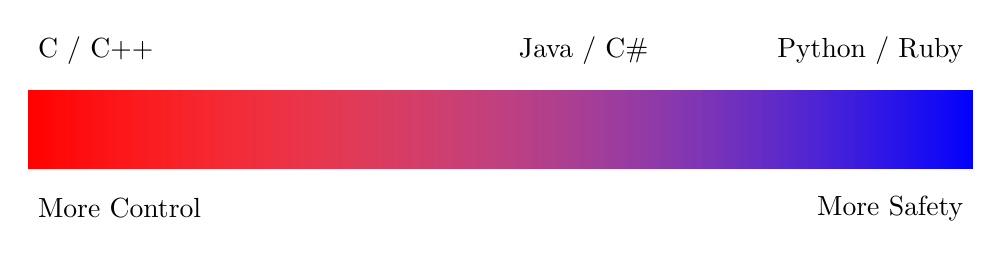
\begin{tikzpicture}
      \fill[blue,path fading=west] (-10:0) rectangle (12,1);
      \fill[red,path fading=east] (-10:0) rectangle (12,1);

      \draw (0,1.5)node[right] {C / C++} ;
      \draw (0,-0.5)node[right] {More Control} ;

      \draw (12,1.5)node[left] {Python / Ruby} ;
      \draw (8,1.5)node[left] {Java / C\#} ;
      \draw (12,-0.5)node[left] {More Safety} ;
    \end{tikzpicture}
    \pause
    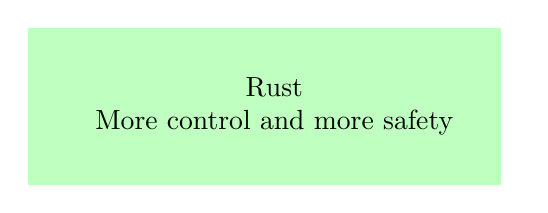
\begin{tikzpicture}
      \fill[ok] (-6:0) rectangle (6,2);
      \draw (0,1)node[right,text width=6cm,align=center]{Rust\\More control and more safety} ;
    \end{tikzpicture}

    \pause \huge{Fast, safe, concurrent, pick three!}
  \end{center}
\end{frame}

%%%

\begin{frame}[c]{A System Programming Language}
  \begin{itemize}
    \item Fine grained control over memory
    \item Close to bare metal
    \item It's possbile to write an OS with it
  \end{itemize}
\end{frame}


\begin{frame}[c]{Blazingly Fast}
  \begin{itemize}
    \item Compiled language
    \item Uses LLVM for optimizations
    \item Zero cost abstractions
  \end{itemize}
\end{frame}


\begin{frame}[c]{Safety}
  \begin{itemize}
    \item No Null pointers
    \item No dangling pointers
    \item No data races
  \end{itemize}
\end{frame}


\begin{frame}[c]{Ownership / Borrowing}
  \begin{itemize}
    \item Every resource has \emph{one owner}
    \item Variables are \emph{moved} to new locations
    \item Owned values can be \emph{borrowd}
      \begin{itemize}
        \item{Either: \emph{One mutable} borrow}
        \item{Or: \emph{Many immutable} borrows}
      \end{itemize}
    \item These rules are enforced by the compiler
  \end{itemize}
\end{frame}

\begin{frame}[c]{Cargo -- Rusts Package Manager}
  \begin{itemize}
    \item Awesome project and package manager
    \item Fetches and builds your project’s dependencies
    \item Invokes rustc or another build tool with the correct parameters
      to build your project
    \item OSS packages on \url{https://crates.io} are immutable\\ $\rightarrow$
      No leftpad like disasters
  \end{itemize}
\end{frame}


\begin{frame}[c]{Community}
  \begin{itemize}
    \item Rust is known for its friendly and welcoming community
    \item The language is develop in the open through RFCs
    \item Active discussion on Github, Reddit, IRC, and the forum
  \end{itemize}
\end{frame}


\begin{frame}[fragile]{Code}
  When including minted code, the \texttt{[fragile]} option needs to be added to
  the frame.

  \begin{minted}{rust}
  let color = Color::Red;
  match color {
    Color::Red => println!("Got red"),
    Color::Green => println!("Got green"),
    Color::Blue => println!("Got blue"),
  }
  \end{minted}
\end{frame}

% ----------------------------------------------------------------- %

\section{Section 2}

\begin{frame}{Picture Time}
  Let's add some more text to it.

  And a picture of a cute cat!

  \includegraphics[height=6cm]{cat.jpg}
\end{frame}

% ----------------------------------------------------------------- %

{
\setbeamertemplate{footline}{}
\pgfdeclareimage[width=\paperwidth]{bg}{background-inverted.pdf}
\usebackgroundtemplate{\pgfuseimage{bg}}
\begin{frame}[standout]
  \begin{centering}
    {\Huge Thank you!}\\
    {\normalsize \url{www.coredump.ch}}\\
  \end{centering}
\end{frame}
}

\end{document}
